\section{Herramientas computacionales}
En esta sección se discuten los programas y herramientas utilizadas en el desarrollado de esta memoria (librerías, utilidades y bases de datos).

\subsection{Herramientas de desarrollo y despliegue}
Python se ha consolidado como el lenguaje de programación por excelencia para el desarrollo y despliegue de modelos de aprendizaje automático. Entre los \textit{frameworks} principales destacan TensorFlow y PyTorch, las cuales se caracterizan por su robustez y adaptabilidad a diversas necesidades. Dado que esta memoria consiste en entrenar un modelo de segmentación y no modificar ni diseñar uno nuevo, es recomendable emplear una librería más sencilla para esta tarea.

\begin{table}[htbp]
\centering
\caption[Plataformas de desarrollo en Python para visión por computadora]{Tabla comparativa de distintas plataformas de desarrollo en Python.}
\label{tab:comparativa_plataformas_desarrollo}
\resizebox{\textwidth}{!}{
\begin{tabular}{|l|l|l|l|l|}
\hline
\multicolumn{1}{|c|}{\textbf{Característica}} & \multicolumn{1}{c|}{\textbf{Tensorflow} \cite{TensorFlow,TensorFlow-whitepaper}} & \multicolumn{1}{c|}{\textbf{Pytorch} \cite{Pytorch,Pytorch2}} & \multicolumn{1}{c|}{\textbf{Supergradients} \cite{Supergradients}} & \multicolumn{1}{c|}{\textbf{Ultralytics} \cite{Ultralytics}} \\ \hline
\begin{tabular}[c]{@{}l@{}}Disponibilidad\\ de modelos\end{tabular} & \begin{tabular}[c]{@{}l@{}}\checkmark\hspace{3px} Múltiples modelos\\ y backbones para usar.\\ \checkmark\hspace{3px} Permite customizar y\\ diseñar modelos.\end{tabular} & \begin{tabular}[c]{@{}l@{}}\checkmark\hspace{3px} Multiples modelos\\ y backbones para usar.\\ \checkmark\hspace{3px} El mayor nivel de\\ customización.\end{tabular} & \begin{tabular}[c]{@{}l@{}}\checkmark\hspace{3px} Modelos de pose y de\\ detección.\\ \xmark \hspace{3px} No hay soporte para\\ modelos de segmentación.\end{tabular} & \begin{tabular}[c]{@{}l@{}}\checkmark\hspace{3px} Modelos YOLO\\ para múltiples tareas.\\ \xmark \hspace{3px} Poca a nula\\ customización.\end{tabular} \\ \hline
Entrenamiento & \begin{tabular}[c]{@{}l@{}}\checkmark\hspace{3px} Simple de realizar.\\ \checkmark\hspace{3px} Muy alto nivel de\\ personalización.\end{tabular} & \begin{tabular}[c]{@{}l@{}}\checkmark\hspace{3px} Algo complicado\\ de realizar.\\ \checkmark\hspace{3px} El mayor nivel de\\ personalización.\end{tabular} & \begin{tabular}[c]{@{}l@{}}\checkmark\hspace{3px}Algo complicado\\ de realizar.\\ \checkmark\hspace{3px} Alto nivel de personaliza-\\ ción (en modelos soportados).\end{tabular} & \begin{tabular}[c]{@{}l@{}}\checkmark\hspace{3px} Muy sencillo.\\ \checkmark\hspace{3px} Buen nivel de\\ personalización.\end{tabular} \\ \hline
Validación & \begin{tabular}[c]{@{}l@{}}\checkmark\hspace{3px} Implementación\\ manual.\end{tabular} & \begin{tabular}[c]{@{}l@{}}\checkmark\hspace{3px} Implementación\\ manual.\end{tabular} & \begin{tabular}[c]{@{}l@{}}\checkmark\hspace{3px} Implementación\\ por interfaz.\end{tabular} & \begin{tabular}[c]{@{}l@{}}\checkmark\hspace{3px} Implementación\\ por interfaz.\end{tabular} \\ \hline
\begin{tabular}[c]{@{}l@{}}Exportación\\ con TensorRT\end{tabular} & \checkmark\hspace{3px} Implementado. & \checkmark\hspace{3px} Implementado. & \begin{tabular}[c]{@{}l@{}}\xmark \hspace{3px} Debe implementarse\\ a parte utilizando Pytorch.\end{tabular} & \checkmark\hspace{3px} Wrapp de Pytorch. \\ \hline
Dificultad. & Media & Alta & Media-alta & Fácil \\ \hline
\end{tabular}
}
\end{table}

\subsubsection{Ultralytics}
Ultralytics \cite{Ultralytics} es un \textit{toolkit} construido sobre PyTorch, especializado en la implementación de la familia de modelos YOLO para detección, segmentación y estimación de pose en tiempo real. Proporciona \textit{scripts} listos para usar, configuraciones predeterminadas optimizadas y facilidades para búsqueda de hiperparámetros, exportación a formatos ONNX y TensorRT, y despliegue en dispositivos borde. Su enfoque ligero y modular permite integrarlo fácilmente en \textit{pipelines} de producción donde se requiera alta velocidad de inferencia y versatilidad en el entrenamiento. El mismo equipo de Ultralytics ha desarrollado algunos de los últimos modelos YOLO disponibles, y es esta disponibilidad de dichos modelos, al igual que la facilidad en sus entrenamientos, la razón por la que se decide usar esta biblioteca por sobre otras alternativas ---como SuperGradients.

\subsection{Herramientas de etiquetado}
Para el etiquetado de imagenes se exploraron varias plataformas para determinar cual se acomoda más a las necesidades del proyecto y WildSense ---dada la colaboración con ellos.

\begin{table}[htpb]
\centering
\caption[Plataformas de etiquetado de bases de datos]{Tabla comparativa de distintas plataformas de etiquetado.}
\label{tab:comparativa_plataformas_etiquetado}
\resizebox{\textwidth}{!}{
\begin{tabular}{|l|l|l|l|l|l|}
\hline
\multicolumn{1}{|c|}{\textbf{Plataforma}} & \multicolumn{1}{c|}{\textbf{Bbox}} & \multicolumn{1}{c|}{\textbf{Segmentación}} & \multicolumn{1}{c|}{\textbf{Tracking}} & \multicolumn{1}{c|}{\textbf{Pros}} & \multicolumn{1}{c|}{\textbf{Contras}} \\ \hline
Roboflow \cite{Roboflow} & \begin{tabular}[c]{@{}l@{}}\checkmark\hspace{3px} Manual\\ \xmark \hspace{3px} Asistida\end{tabular} & \begin{tabular}[c]{@{}l@{}}\checkmark\hspace{3px} Manual\\ \checkmark\hspace{3px} Asistida\end{tabular} & \xmark \hspace{3px} No disponible. & \begin{tabular}[c]{@{}l@{}}- Interfaz simple.\\ - Permite entrenar \\ modelos dentro\\ de su plataforma.\end{tabular} & \begin{tabular}[c]{@{}l@{}}- Hay que pagar\\ para tener el\\ dataset privado.\end{tabular} \\ \hline
CVAT \cite{CVAT} & \begin{tabular}[c]{@{}l@{}}\checkmark\hspace{3px} Manual\\ \xmark \hspace{3px} Asistida\end{tabular} & \begin{tabular}[c]{@{}l@{}}\checkmark\hspace{3px} Manual\\ \checkmark\hspace{3px} Asistida\end{tabular} & \begin{tabular}[c]{@{}l@{}}\checkmark\hspace{3px} Manual\\ \checkmark\hspace{3px} Asistida\\ con bbox.\end{tabular} & \begin{tabular}[c]{@{}l@{}}- Intefaz simple.\\ -Puede correr de\\ forma local.\end{tabular} & \begin{tabular}[c]{@{}l@{}}- Puede tener\\ incompatibilidad\\ con Firefox.\\ - Segmentación\\ asistida lenta.\end{tabular} \\ \hline
V7 Labs \cite{V7Labs} & \begin{tabular}[c]{@{}l@{}}\checkmark\hspace{3px} Manual\\ \checkmark\hspace{3px} Asistida\end{tabular} & \begin{tabular}[c]{@{}l@{}}\checkmark\hspace{3px} Manual\\ \checkmark\hspace{3px} Asistida\end{tabular} & \begin{tabular}[c]{@{}l@{}}\checkmark\hspace{3px} Manual\\ \checkmark\hspace{3px} Asistida\\ con segmentación.\end{tabular} & \begin{tabular}[c]{@{}l@{}}- Permite entrenar\\ modelos dentro\\ de su plataforma.\end{tabular} & \begin{tabular}[c]{@{}l@{}}- Interfaz muy\\ lenta y con lag.\end{tabular} \\ \hline
Labellerr \cite{Labellerr} & \begin{tabular}[c]{@{}l@{}}\checkmark\hspace{3px} Manual\\ \checkmark\hspace{3px} Asistida\end{tabular} & \begin{tabular}[c]{@{}l@{}}\checkmark\hspace{3px} Manual\\ \checkmark\hspace{3px} Asistida\end{tabular} & \begin{tabular}[c]{@{}l@{}}\checkmark\hspace{3px} Manual\\ \xmark \hspace{3px} Asistida\end{tabular} & \begin{tabular}[c]{@{}l@{}}- Permite entrenar\\ modelos dentro de\\ su plataforma.\end{tabular} & \begin{tabular}[c]{@{}l@{}}- Interfaz\\ complicada y\\ difícil de usar.\end{tabular} \\ \hline
Supervisely \cite{Supervisely} & \begin{tabular}[c]{@{}l@{}}\checkmark\hspace{3px} Manual\\ \checkmark\hspace{3px} Asistida\end{tabular} & \begin{tabular}[c]{@{}l@{}}\checkmark\hspace{3px} Manual\\ \checkmark\hspace{3px} Asistida\end{tabular} & \begin{tabular}[c]{@{}l@{}}\checkmark\hspace{3px} Manual\\ \checkmark\hspace{3px} Asistida\end{tabular} & \begin{tabular}[c]{@{}l@{}}- Múltiples apps\\ y opciones para\\ los proyectos.\end{tabular} & \begin{tabular}[c]{@{}l@{}}- Tracking\\ asistido lento.\end{tabular} \\ \hline
SAM2 \cite{SAM2} & \checkmark\hspace{3px} Asistida & \checkmark\hspace{3px} Asistida & \checkmark\hspace{3px} Asistida & \begin{tabular}[c]{@{}l@{}}- Se ejecuta\\ localmente\end{tabular} & \begin{tabular}[c]{@{}l@{}}- Implementación\\ manual.\\- Requiere GPU.\end{tabular} \\ \hline
\end{tabular}
}
\end{table}

\subsubsection{CVAT}
\textit{Computer Vision Annotation Tool} (CVAT) \cite{CVAT} es una herramienta de código abierto diseñada para facilitar la anotación de imágenes y videos. Soporta la creación de cajas englobantes, polígonos, y \textit{keypoints} de manera manual, así como la segmentación de instancias y seguimiento de objetos en videos, de forma manual y asistida. CVAT es conocido por su simplicidad y velocidad, lo que lo convierte en una opción ideal para proyectos que requieren anotaciones precisas.

\subsubsection{Roboflow}
Roboflow \cite{Roboflow} es una plataforma de anotación de imágenes para tareas de inteligencia artifical con especial enfoque en la facilidad de despliegue y exportación. Lamentablemente no posee utilidades para el etiquetado en \textit{tracking} y por defecto sus bases de datos son públicas, con la alternativa privada requiriendo un pago anual fuera de cualquier presupuesto razonable para esta memoria.

\subsection{Bases de datos}
Para el entrenamiento de los modelos se utilizaron dos bases de datos de segmentación de instancias. El primero de carácter público y con la finalidad de replicación de resultados. El segundo de carácter privado, que además es depurado en una versión más refinada para lograr mejores modelos.

\begin{table}[htbp]
\centering
\caption[Detalles de la composición de las bases de datos de segmentación]{Detalles con el número de imágenes y etiquetas para las bases de datos Deepfish y Salmons. Las variantes ``\_LO'' corresponden a los mismos \textit{datasets} pero sin imágenes de fondo en la tarea de entrenamiento.}
\label{tab:datasets_combined}
\begin{tabular}{|c|c|c|c|c|}
\hline
\textbf{Dataset} & \textbf{Tarea} & \textbf{Num. imgs.} & \textbf{Num. segm.} & \textbf{Img. fondo} \\ \hline
\multirow{4}{*}{\begin{tabular}[c]{@{}c@{}}Deepfish\\ (620)\end{tabular}} & Train & 309 & 182 & 161 \\ \cline{2-5} 
 & Validation & 125 & 79 & 59 \\ \cline{2-5} 
 & Testing & 186 & 113 & 90 \\ \cline{2-5} 
 & Total & 620 & 374 & 310 \\ \hline
\multirow{4}{*}{\begin{tabular}[c]{@{}c@{}}Deepfish\_LO\\ (459)\end{tabular}} & Train & 148 & 182 & 0 \\ \cline{2-5} 
 & Validation & 125 & 79 & 59 \\ \cline{2-5} 
 & Testing & 186 & 113 & 90 \\ \cline{2-5} 
 & Total & 459 & 374 & 149 \\ \hline
\multirow{4}{*}{\begin{tabular}[c]{@{}c@{}}Salmons\\ (1280)\end{tabular}} & Train & 1109 & 2429 & 524 \\ \cline{2-5} 
 & Validation & 154 & 428 & 26 \\ \cline{2-5} 
 & Testing & 17 & 57 & 0 \\ \cline{2-5} 
 & Total & 1280 & 2914 & 550 \\ \hline
\multirow{4}{*}{\begin{tabular}[c]{@{}c@{}}Salmons\_LO\\ (756)\end{tabular}} & Train & 585 & 2429 & 0 \\ \cline{2-5} 
 & Validation & 154 & 428 & 26 \\ \cline{2-5} 
 & Testing & 17 & 57 & 0 \\ \cline{2-5} 
 & Total & 756 & 2914 & 550 \\ \hline
\end{tabular}
\end{table}

Finalmente se utilizó una base de datos de seguimiento para la validación en esa tarea de los modelos entrenados para salmones.

\begin{table}[htbp]
\centering
\caption[Composición de las bases de datos de seguimiento]{Composición de las bases de datos de seguimiento.}
\label{tab:datasets_tracking}
\begin{tabular}{|l|l|l|l|l|}
\hline
\textbf{Dataset} & \textbf{Cuadros} & \textbf{IDs} & \textbf{Bboxes} & \textbf{Descripción} \\ \hline
Video\_1 & 220 & 36 & 2039 & Aguas verdes con buena visibilidad. \\ \hline
Video\_2 & 220 & 37 & 1855 & Aguas azules con baja visibilidad. \\ \hline
\end{tabular}
\end{table}

\begin{figure}[htbp]
    \centerline{
    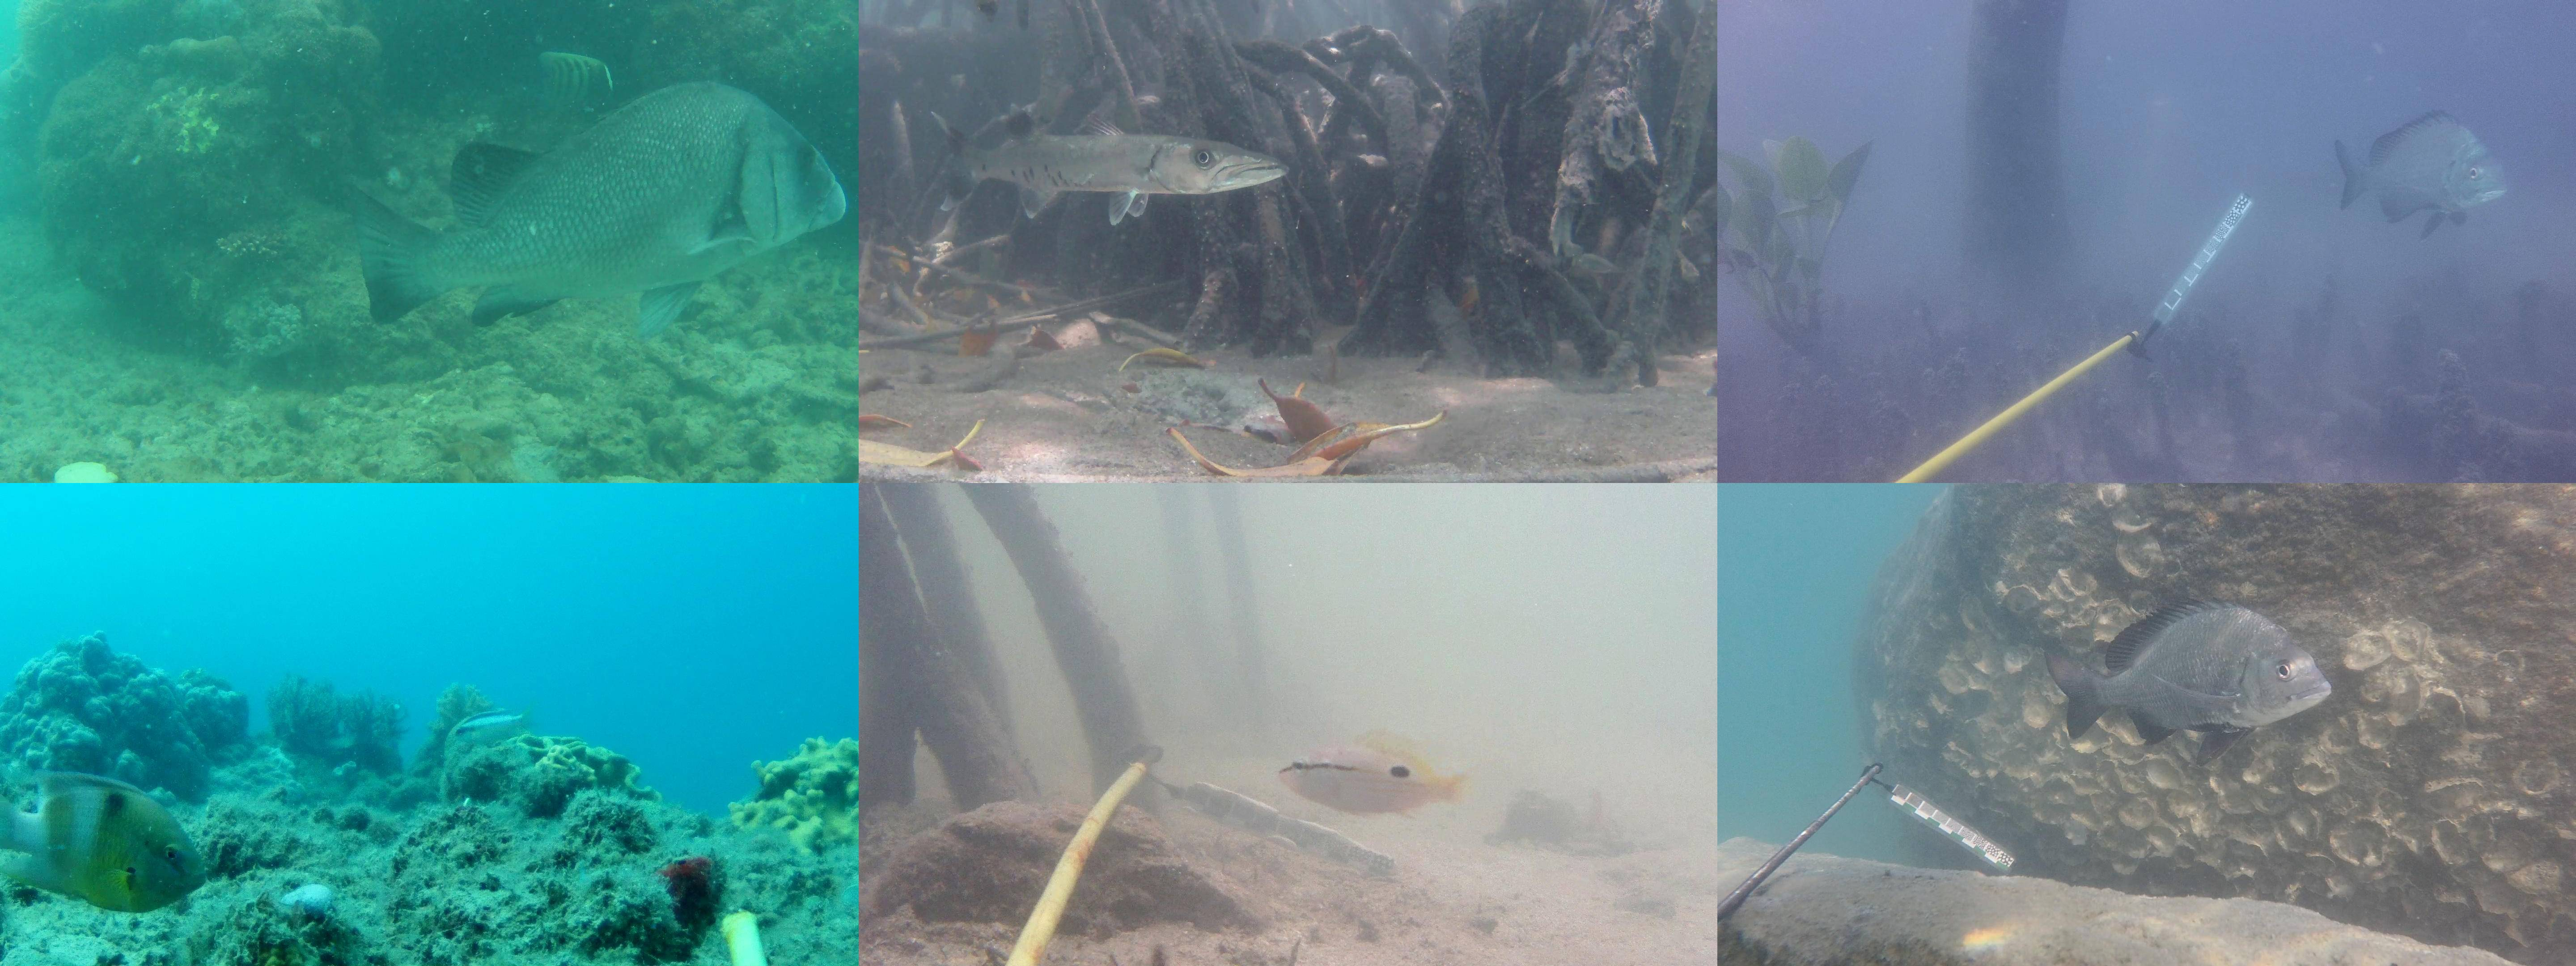
\includegraphics[width=.9\linewidth]{figures/deepfish_muestra.jpg}}
    \caption[Muestra de la base de datos Deepfish]{Muestra de imágenes de la base de datos Deepfish.}
    \label{deepfish_muestra}
\end{figure}

\begin{figure}[htbp]
    \centerline{
    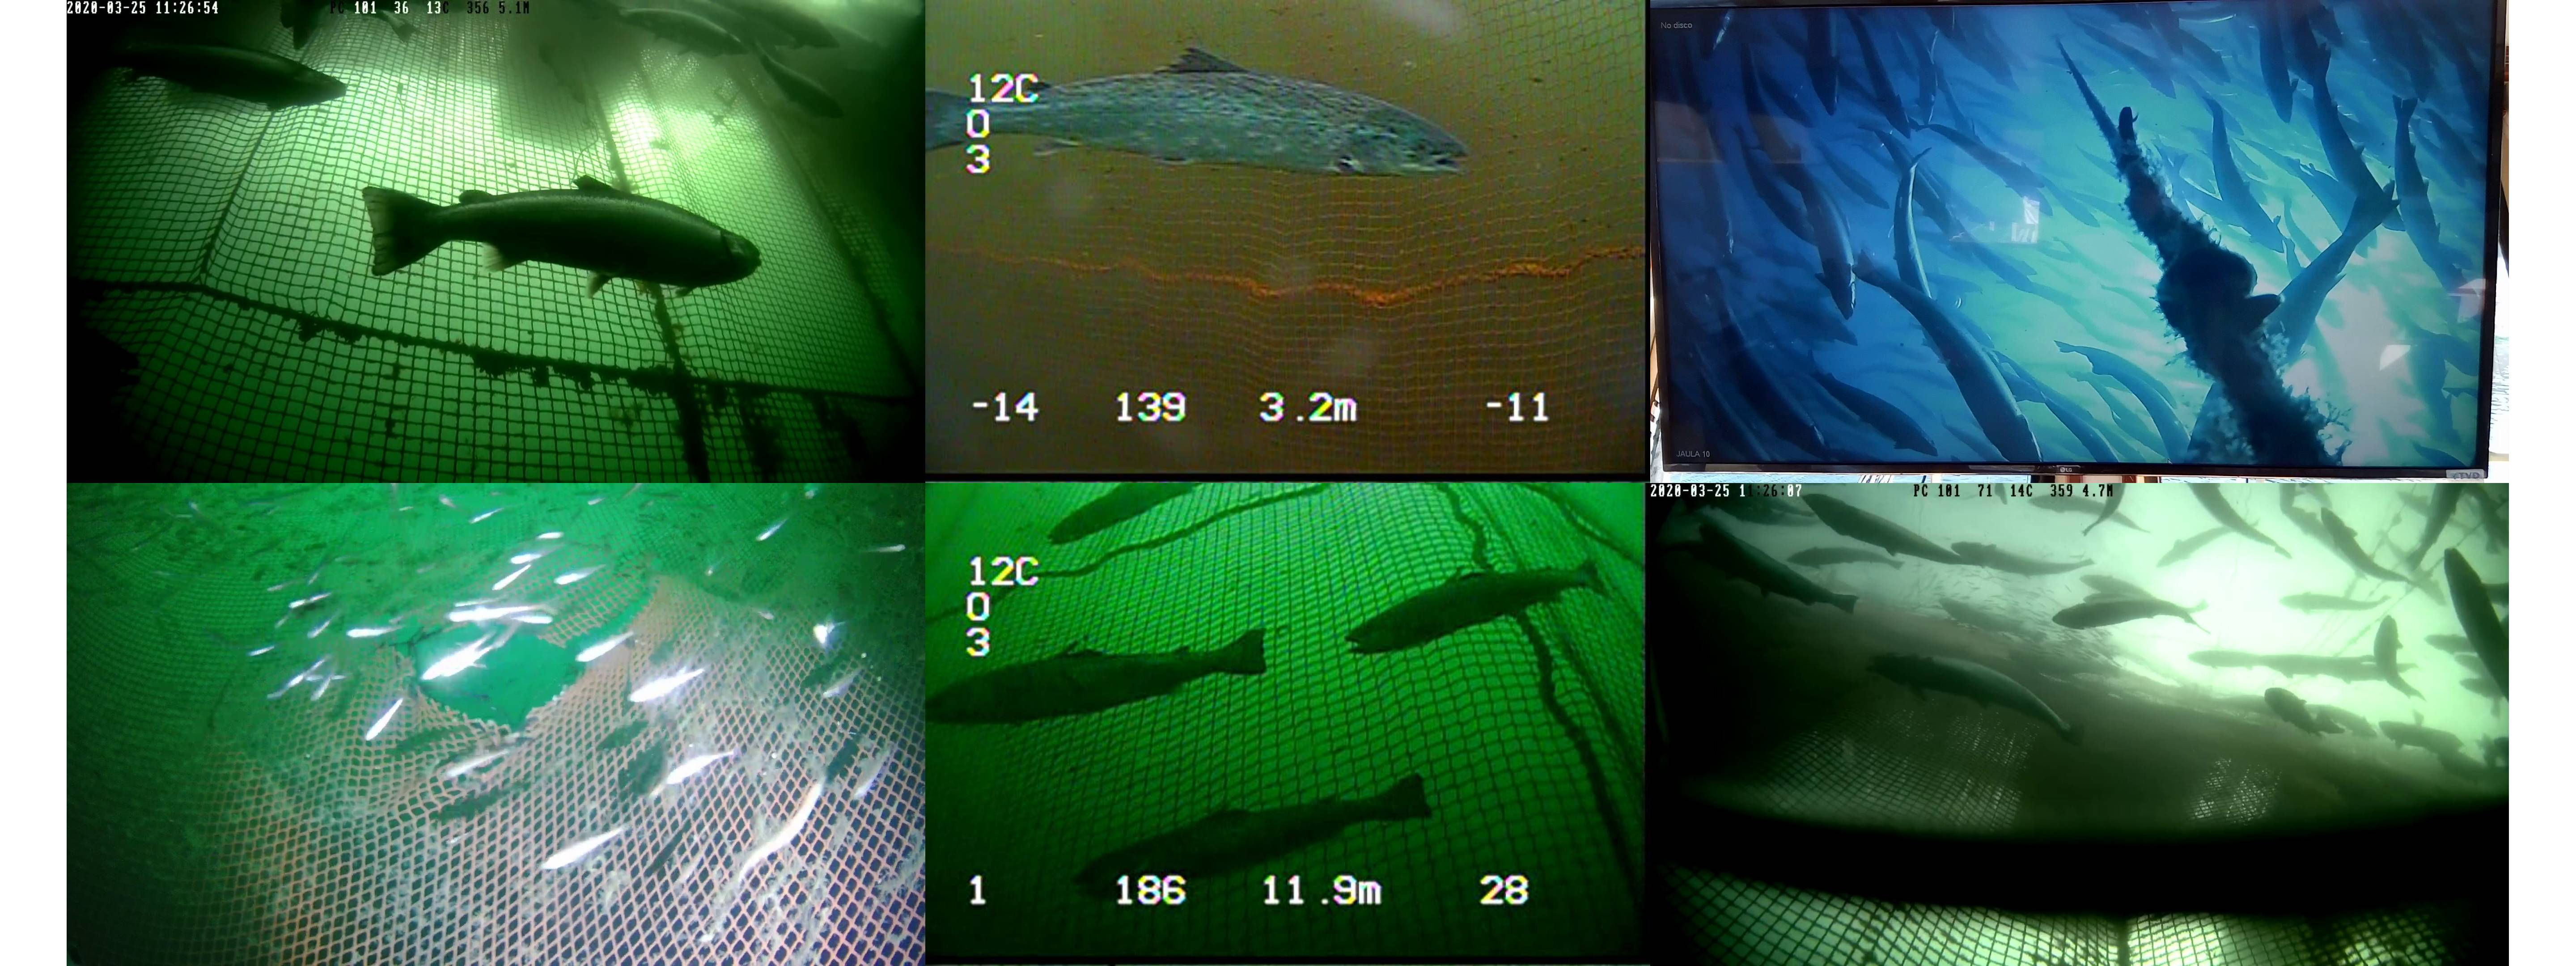
\includegraphics[width=.9\linewidth]{figures/salmon_muestra.jpg}}
    \caption[Muestra de la base de datos Salmons]{Muestra de imágenes de la base de datos Salmons.}
    \label{salmon_muestra}
\end{figure}

\begin{figure}[htbp]
    \centerline{
    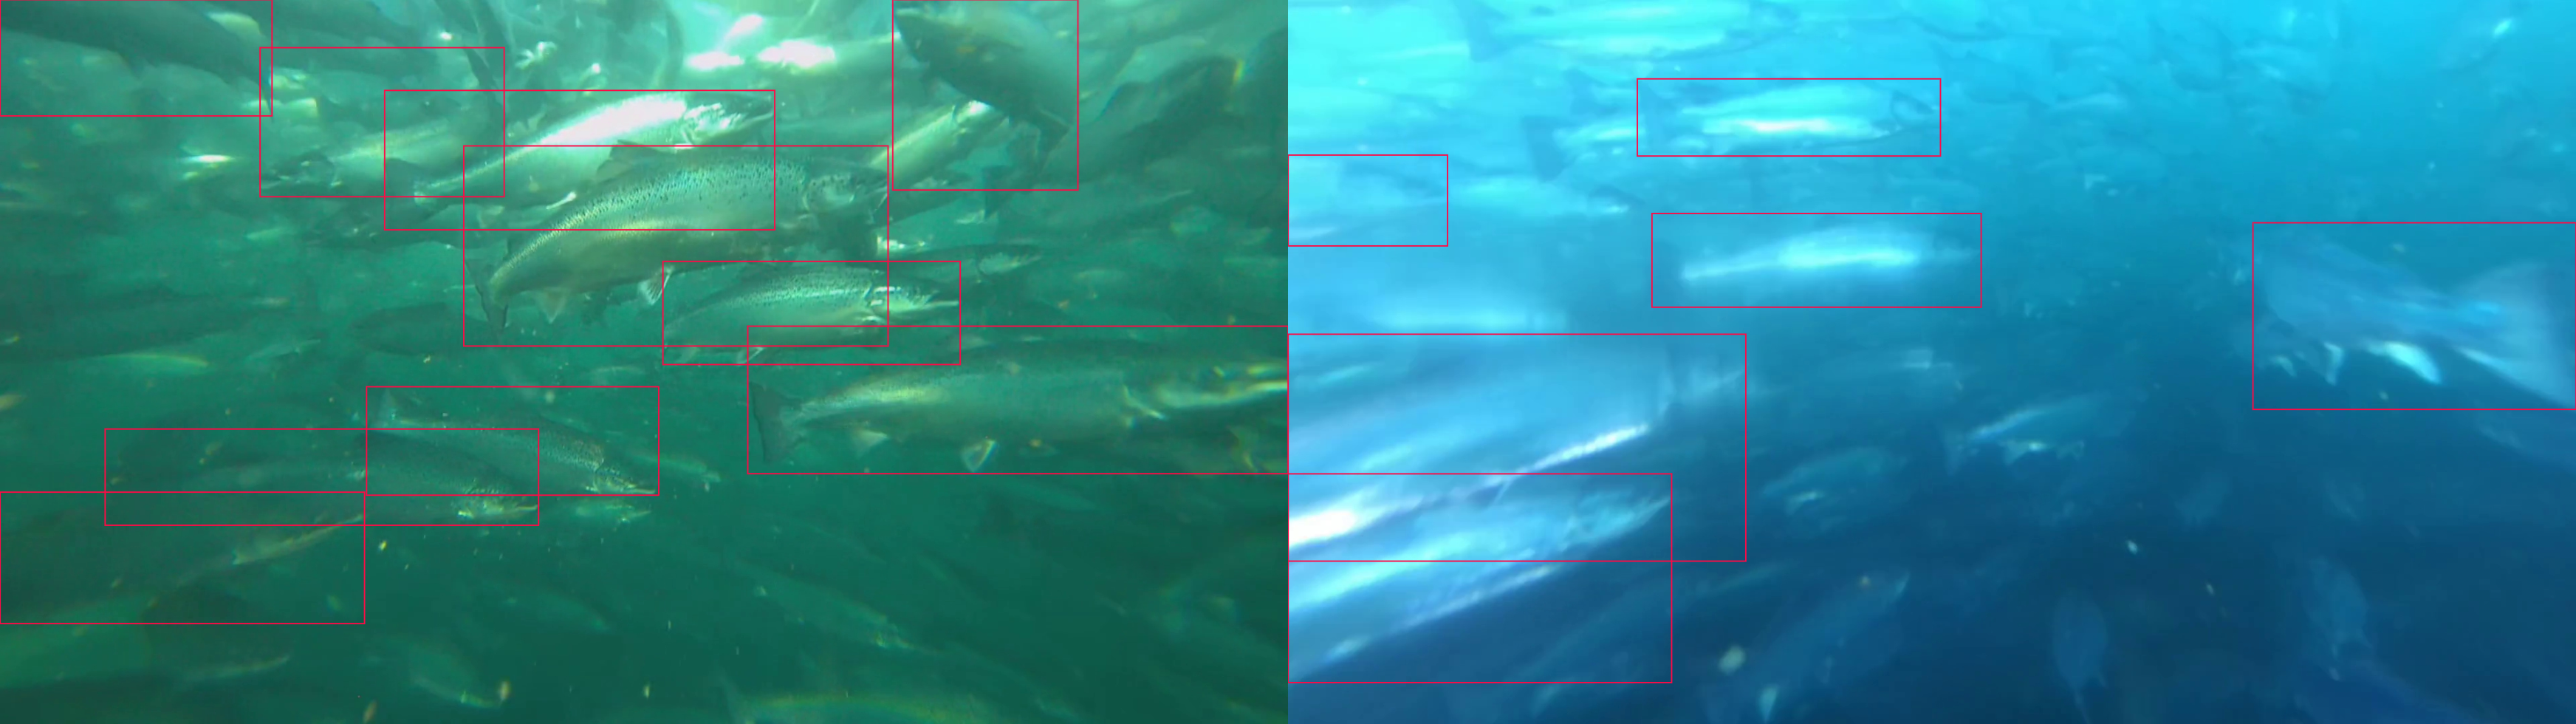
\includegraphics[width=.9\linewidth]{figures/Muestras_video.png}}
    \caption[Muestra de la base de datos de seguimiento]{Muestra de imágenes de la base de datos de seguimiento.}
    \label{tracking_muestra}
\end{figure}

\subsubsection{Deepfish}
Esta base de datos de dominio público fue desarrollada como un \textit{benchmark} para tareas de clasificación con peces, etiquetando en variados contextos y habitats \cite{Deepfish}. Para este trabajo solo se utilizaron las etiquetas e imágenes en la tarea de segmentación de instancias, pero el \textit{dataset} completo también contempla otras tareas de clasificación. Para el despliegue del mismo se utilizó una versión trabajada con anterioridad disponible desde Roboflow \cite{DeepfishRoboflow}.

\subsubsection{Salmons}
Esta base de datos es una versión optimizada del dataset de salmones desarrollado por WildSense y es de caracter privado. Para el desarrollo de este se utilizó como punto de partida la base de datos ``Salmons_2024base'', disponible en el espacio de trabajo de WildSense en CVAT. Luego de depurar instancias de no interés, se procedió a incluir 321 imágenes de los \textit{dataset} de \textit{tracking} con segmentación llamadas ``Seguimiento_1'' y ``Seguimiento_2'', también disponibles desde el mismo espacio de trabajo en CVAT.

\subsubsection{Tracking Salmones}
Esta base de datos corresponde a dos videos de 220 cuadros cada uno y las etiquetas están en forma de cajas englobantes.
